\documentclass[12pt, letterpaper]{report}
\usepackage[spanish, es-tabla]{babel}% coloca tabla en lugar de cudro en las tablas e idioma español.
% Dimensiones y márgenes---------------------------------------------
\usepackage[total={18cm,21cm},top=4cm, left=2cm, right = 3 cm]{geometry}
\usepackage[scaled]{helvet}
\renewcommand*\familydefault{\sfdefault} 
%\usepackage[T1]{fontenc}
% Otros paquetes -----------------------------------------------------
\usepackage{mathpazo} %fuente palatino
\usepackage{graphicx} %paquete para gáficos
%\usepackage{xcolor}	%paquete para colores
\usepackage{pstricks}	
\usepackage[utf8]{inputenc}
%\usepackage[shortlabels]{enumitem}
% Referencias para graficos
\usepackage{graphicx} % gráficos
\usepackage{subfigure} % subgráficos
% Referencias - ligas
\usepackage[hyphens]{url}
\usepackage[breaklinks,colorlinks=true,linkcolor=red, citecolor=red, urlcolor=blue]{hyperref}
%Paquetes adicionales de símbolos matemáticos
\usepackage{amsmath,amssymb,cancel}% funciones matematicas ,amsfonts ,latexsym
%Comandos ---------------------------------------------------------
\usepackage{fix-cm} % Allows increasing the font size of specific fonts beyond 
\usepackage{colortbl} % Comandos personales - especiales
\usepackage{ multirow, array} % para las tablas
\usepackage{float} % para usar [H]
\usepackage{longtable} % para tablas largas
%\pagestyle{empty}
\usepackage{booktabs}
\usepackage{fancyhdr}
\usepackage{rotating}% paquete para rotar
%\usepackage{html,makeidx}
%\usepackage{cite}
%\pagestyle{myheadings}% estilo de pagina propio
%\markright{\rightmark} %\usepackage{fancyhdr}% para los estilos de encabezado y pie de pagina
\pagestyle{fancy}% estilo de pagina
%\fancyfoot[LE,RO]{\thepage}
% cabecera y pie
\lhead{Página \thepage } % texto izquierda de la cabecera
%\chead{TEXTO} % texto centro de la cabecera
%\rhead{\thepage} % número de página a la derecha
\lfoot{} % texto izquierda del pie
%\cfoot{\includegraphics[width = 1cm]{universidad.png} } % imagen centro del pie
%\rfoot{ \textit{Maestria en Ingenieria con Énfasis en Ing. Eléctrica}} % texto derecha del pie
%\renewcommand{\headrulewidth}{0.4pt} % grosor de la línea de la cabecera
%\renewcommand{\footrulewidth}{0.4pt} % grosor de la línea del pie
%LaTeX default specifications
%more content to this template

\definecolor{grey}{rgb}{0.9,0.9,0.9} % Color of the box surrounding the title - these values can be changed to give the box a different color	


\begin{document}
\title{tesis}
\author{Alejandro Palacios Carabali.}
\date{2017}
%\tableofcontents
%----------------------------------------------------------------------------------------
%	TITLE SECTION
%---------------------------------------------------------
\thispagestyle{empty}% pagina no numerada	
\colorbox{grey}{
	\parbox[t]{1.0\linewidth}{
		\centering \fontsize{20pt}{30pt}\selectfont % The first argument for fontsize is the font size of the text and the second is the line spacing - you may need to play with these for your particular title
		\vspace*{0.7cm} % Space between the start of the title and the top of the grey box
		
		\hfill \textbf{ ESTADO DEL ARTE}\\ 
		\hfill \textbf{SOBRE }\\
		\hfill \textbf{ESTRATEGIAS }\\
		\hfill \textbf{PARA LA REGULACIÓN DE} \\
		\hfill \textbf{VOLTAJE EN REDES DE } \\ 
		\hfill \textbf{DISTRIBUCIÓN ELÉCTRICA } \\ 
		\hfill \textbf{CON ALTO GRADO DE}\\
		\hfill \textbf{GENERACIÓN }\\
		\hfill \textbf{DISTRIBUIDA }\\
		\hfill \textbf{RENOVABLE }\\
		\par
		
		\vspace*{0.7cm} % Space between the end of the title and the bottom of the grey box
	}
}

%----------------------------------------------------------------------------------------

\vfill % Space between the title box and author information

%----------------------------------------------------------------------------------------
%	AUTHOR NAME AND INFORMATION SECTION
%----------------------------------------------------------------------------------------

{\centering \large 
\hfill Alejandro Palacios \\
\hfill Universidad del Valle \\
\hfill Escuela de Ingeniería Eléctrica y Electrónica \\
\hfill Directores:\\
\hfill Diego Fernando Echeverry\\
\hfill Sandra Milena Londoño\\

}
%{1pt}} % Horizotal line, thickness changed here

%----------------------------------------------------------------------------------------
\sloppy
\chapter*{INTRODUCCIÓN}
Los \textit{sistemas de distribución eléctrica} (DS \textit{Distribution System} ) son la ultima etapa en el transporte de energía eléctrica  desde los generadores hasta los \textit{usuarios finales} dentro del sistema eléctrico de potencia (EPS  \textit{electrical power system}) \cite{basso2004ieee}. La electricidad transportada a través de los DS en las dos décadas anteriores se ha caracterizado por provenir en mayor grado fuentes hidráulicas, nucleares y  fósiles ( como carbón, petroleo, gas, etc) \cite{Bacha2015}. Estas ultimas al ser empleadas tanto para la generación eléctrica como en es sector del transporte \cite{Bahmanifirouzi2012} han traído como consecuencia un incremento del calentamiento global a raíz  de los gases de efecto invernadero que se liberan en  su proceso de combustión  \cite{Hauck2017}.\\\\
Como respuesta a esta problemática en los años recientes se ha dado  paso al incremento de la generación a pequeña  escala instalada dentro del DS conocida como generación distribuida  (DG \textit{Distributed Generation}) ya sea de carácter renovable  (Renewable Energy Sources RES) como la fotovoltaica, solar térmica, eólica, biomasa y micro turbinas hidráulicas  \cite{Calderaro2014} o no renovable. Algunas de estas fuentes renovables son intermitentes y su generación depende de condiciones ambientales \cite{Mahmud2016}. Esto causa problemas de estabilidad, confiabilidad, aumento en las perdidas y mala \textit{calidad de energía} \cite{Karanki2014}\cite{DinakaraPrasadReddy2017}.\\\\ 
Entre los parámetros más importantes de  calidad de la energía se encuentra el \textit{nivel de tensión}, el cual se ve afectado por los flujos de potencia bidireccionales \cite{Koutsoukis2017}, la ubicación de la GD \cite{Othman2016a}, la topologia de la red y las impedancias del DS .  En este trabajo se abarcan las soluciones mas destacadas  para realizar el control de la tensión en un DS cuando hay presencia de DG de tipo RES. \\\\
En el capitulo \ref{cap_oltc} trata del control de tensión a través de un cambiador de tomas, en el capítulo \ref{cap_reactiva} se trata del control de tensión mediante el control del flujo de potencia reactiva esto  a través de la gestión de bancos de condensadores, en el capítulo \ref{cap_almacenamiento} hace referencia al impacto del almacenamiento de energía en el control de tensión, en el capítulo \ref{cap_inversor} se enfoca en los algoritmos construidos  en los inversores  de la DG para el control de tesnión, en el capítulo \ref{cap_central} hace referencia  a las comunicaciones y su influencia  y finalmente en el capítulo \ref{cap_planeacion} trata sobre la localización optima de DG para el control de tensión.\\\\

\chapter{IMPACTO EN LA TENSIÓN DEBIDO AL INCREMENTO EN LA DE GENERACIÓN DISTRIBUIDA EN LA RED DE DISTRIBUCIÓN}
Los sistemas de distribución modernos han sido diseñados para recibir grandes cantidades de potencia y transmitirla de manera vertical\cite{Badran2017}, empleando para ello la red de transmisión, la de  de sub transmisión y finalmente el DS, conformado este ultimo por la red de media tensión ( \textit{medium voltage} MV ) y la de baja tensión ( \textit{low voltage} LV ) \cite{Tang2017} consiguiendo así suplir los usuarios finales \cite{Delfanti2013}. Sin embargo con el crecimiento de la GD en los DS se ha dado lugar a la aparición de flujos de potencia inversos (desde la carga hacia el DS) lo cual acompañado por los altos valores en la relación R/X (resistencia reactancia) principalmente en los circuitos de LV, dan lugar a la aparición de sobre tensiones en los nodos del  DS \cite{su2009comparative}\cite{Tang2017}.\\\\
Para ilustrar este fenómeno se parte  del diagrama unifilar de la figura \ref{fig:dos_nodos} en el que se representan las características básicas de un sistema de potencia con GD. Este esta conformado por la carga que demanda una potencia $P_{L}+jQ_{L}$, la DG que genera o absorbe una potencia $P_{DG}\pm jQ_{DG}$,  la compensación reactiva que inyecta o absorbe una potencia $\pm jQ_{C}$, la impedancia de linea $R+jX$,  los nodos $V_{i} $ de entrada y $V_{DG}$ en la carga y el equivalente de red del sistema.\\\\

%El abseso a la electricidad suministrado a la población global  en las dos ultimas decadas  se ha caracterizado por estar dirigido en mayor grado al sector urbano frente al correpondiente sector rural\cite{Bowman2017}. Este fenomeno de dezplazamiento de la poblacion hacia las ciudades lo que ha ocacionado  un \textit{incremento en la demanda de electricidad}. Este echo unido al calentamiento global causado principalmente por los gases de efecto invernadero \cite{Hauck2017} producto en parte de la generación electrica  a partir de materiales fósiles ( como carbón, petroleo, gas, etc)  han dado  paso al incremento de la generación a pequeña  escala o generación distribuida (DG \textit{Distributed Generation}) de caracter renovable dentro de los sistemas de distribución de energia electrica (DPS \textit{Distribution Power System}) en dichas áreas urbanas. \\\\
%Este tipo de  fuentes renovables tienen la particularidad de ser utilizadas tanto en grandes centros de consumo, como en pequeñas micro - generaciones principalmente dentro de   las instalaciones del usuario final (autogeneración) \cite{manfren2011paradigm}.
%Estas fuentes de DG se pueden clasificar de acuerdo a su recurso primario como: fotovoltaicas, eólicas, microturbinas hidraulicas, microturbinas a gas, celdas de conbustion, maquinas reversibles, generación con diesel y gas natural y almacenamiento de energia \cite{Emmanuel2017a}\cite{puttgen2003distributed}. 
\begin{figure}[h]
    \centering
    \caption{Diagrama unifilar de una red simplificada}
    \label{fig:dos_nodos}
    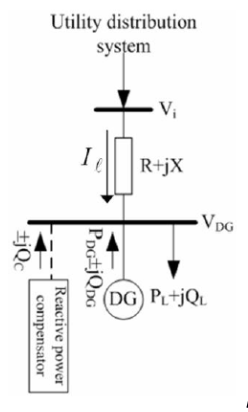
\includegraphics[width=0.4\linewidth]{imagenes/cap_1/dos_nodos}
\end{figure}
De acuerdo a la definición de potencia compleja se tiene la siguiente expresión \cite{Akagi1932}:

\begin{equation}
\label{equ:comp}
P + jQ = V_{DG} \cdot I_{l}^{*}
\end{equation}
De la ecuación \ref{equ:comp}  se puede obtener  la corriente de línea en función de la potencia activa y reactiva :

\begin{equation}
I_{l}= \dfrac{P + jQ}{\overrightarrow{V_{DG}^{*}}}
\label{eq:corriente}
\end{equation}

Aplicando el la ley de \textit{ Kirchoff } de tensiones en el nono  $V_{GD}$, este  puede ser expresado como:\\\\
\begin{equation}
\label{equ:volt_gd}
\overrightarrow{V_{DG}}= \overrightarrow{V_{i}} + I_{l}(R + X_{L})
\end{equation}

Remplazando $ I_{l} $ de  la ecuación \ref{eq:corriente} en la ecuación  \ref{equ:volt_gd} se tiene:

\[\overrightarrow{V_{DG}}= \overrightarrow{V_{i}} + \dfrac{P + jQ}{\overrightarrow{V_{DG}^{*}}}(R + X_{L})\]
\begin{equation}
\overrightarrow{V_{DG}}= \overrightarrow{V_{i}} + \dfrac{RP + X_{l}Q}{\overrightarrow{V_{DG}^{*}}} + j\dfrac{RP - X_{l}Q }{\overrightarrow{V_{DG}^{*}}}
\end{equation}

Cuando el ángulo entre los fasores de tensión  $V_{DG}$  y $V_{l}$ es pequeño, es decir cuando la potencia activa entregada por el $DS$ tiende a cero \cite{Akagi1932} (  esto puede darse porque no hay demanda de energía o la $DG$ abastece la demanda de la carga en una condición de auto consumo de los usuarios o de la micro red), y si además de ello se considera el voltaje en el nodo $V_{DG}$ como referencia fasorial (ángulo 0) la caída de tensión en la línea puede ser escrita como:\\\\
\begin{equation}
\Delta\ V \cong V_{DG} - V_{i}\cong \dfrac{RP - X_{l}Q }{V_{DG}}
\label{eq:delta} 
\end{equation}
Donde, $\Delta V$ es la caída de tensión a través del alimentador. Si también asumimos que la tensión en el nodo  $V_{DG}$  es la tensión base, entonces podemos reescribir la ecuación \ref{eq:delta} como:\\\\
\begin{equation}
\Delta\ V \cong V_{DG} - V_{i}\cong RP - X_{l}Q 
\label{eq:delta1} 
\end{equation}
Donde $P=(P_{DG}-P_{L})$  y  $ Q = (\pm Q_{DG} \pm Q_{c} - Q_{L})$.\\\\
De este modo la ecuación \ref{eq:delta1} puede ser reescrita así:

\begin{equation}
V_{DG} \cong V_{i} + R (P_{DG} - P_{L}) + X(\pm Q_{DG} \pm Q_{c} - Q_{L})
\label{eq:voltajeds}
\end{equation}
De este modo  de la ecuación \ref{eq:voltajeds} se puede determinar  el nivel máximo de generación que puede  albergar un circuito.\\\\
Para tal caso se plantean dos escenarios críticos en los cuales se presentan las máximas desviaciones de tensión \cite{Elkhatib2011}:\\\\

\begin{tabular}{|c|c|c|}
    \hline 
    Caso 	& Carga 	& Generación \\\hline
    1 		& Mínima	& Máxima \\\hline
    2		& Máxima	& Máxima \\
    \hline
\end{tabular}

\section{Caso crítico ( carga mínima  y máxima generación ) }
Se considera este primer escenario en el cual la demanda de la carga es mínima, por ejemplo  para una carga residencial típica  esto es  en las horas de medio día  o en la madrugada. La otra condición de máxima generación se presenta por ejemplo para fuentes fotovoltaicas  en el medio día,  con lo cual se podría tener que para un caso típico de carga residencial con generación fotovoltaica esta condición se alcanzaría en medio día.\\\\
Esto se puede  cuantificar a partir de la ecuación \ref{eq:voltajeds} se tenga un factor de potencia igual a uno  en el nodo  $V_{DG}$, entonces se puede deducir que la máxima tensión en este nodo se obtiene cuando hay la mínima carga ($P_{L} = 0$ , $Q_{L} = 0$ )  y la generación máxima ($P_{G} = P_{GMAX}$). En estas condiciones el OR puede operar incluso sin que exista generación distribuida. la tensión en el nodo $V_{DG}$, queda determinado entonces por la ecuación \ref{eq:voltajeds} así \cite{strbac2002integration} :\\\\
\begin{equation}
V_{DG} = V_{i} + P_{GMAX}
\label{eq:vgmax}
\end{equation}


\begin{tabular}{l c r}
    & &\\
    Donde:& & \\
    & &\\
    & $P_{GMAX}$ & Es la potencia máxima permisible en el DS.\\
    & &\\
    & &\\
\end{tabular}\\\\
En estas condiciones la potencia máxima permisible en el sistema es :\\\\
\begin{equation}
P_{GMAX} \leq \frac{V_{DGMAX} - V_{i}}{R}
\label{eq:pgmax}
\end{equation}
\begin{tabular}{l c r}
    & &\\
    Donde:& & \\
    & &\\
    & $V_{DGMAX}$ & Es la tensión máxima permisible en el DS.\\
    & &\\
    & &\\
\end{tabular}\\\\
Se puede notar en la ecuación \ref{eq:pgmax} la potencia máxima generada es función de la resistencia de línea, de modo tal que la resistencia de la linea ( que depende del calibre del conductor y la longitud ) determina la máxima potencia que puede ser inyectada al sistema.\\\\
\section{Caso critico máxima carga y mínima generación }
Se considera este segundo escenario en el cual la demanda es alta , por ejemplo  para una carga residencial típica  esto es  en el inicio de la noche o iniciando la mañana y ademas la generación producida por los diferentes DS es baja.\\\\
Considerando igualmente un factor de potencia unitario por tanto la ecuación \ref{eq:voltajeds} puede ser  escrita para este caso así:

\[V_{DG} = V_{i} - RP_{Lmax}\]

O

\[P_{Lmax} = \dfrac{V_{i} - V_{DG }}{R}\]

Consideremos ahora que $V_{DGmin}$ es el mínimo voltaje permisible en el DS. Por tanto para mantener el voltaje bajo los limites permisibles  se debe cumplir que:

\[P_{Lmax} \leq \dfrac{V_{i} - V_{DGmin}}{R}\]

Otro factor importante   el el factor $ R/X $ donde $ R $ es la resistencia  del equivalente thevenin de la figura.
\section{Dependencia del factor R/X}
Otro indicador importante al momento de establecer el control de tensión es el factor $ R/X$ del equivalente de red, donde $R$  y $X$ son respectivamente la resistencia y la reactancia  \textit{Thevenin} del EPS en el nodo $V_{GD}$.    Para \textit{valores bajos} del parámetro $R/X$ ( es decir donde el equivalente de red es principalmente reactivo ) la potencia activa tiene muy poca  influencia en los perfiles de tensión, mientras conforme el parámetro $R/X$ crece, el efecto de la potencia activa sobre las tensiones es mas determinante. Dicho de otro modo, en \textit{media tensión } y baja tensión la inyección de potencia activa por parte de la GD provoca aumentos de la tensión en el PCC.\\\\
De algún modo este efecto de la potencia activa en los niveles de tensión debe ser mantener la tensión en el punto de nominal compensado mediante la absorción de potencia reactiva para devolver los niveles de tensión a su condición de diseño.\\\\
La potencia reactiva necesaria para mantener la tensión en el nodo $ V_{DG}$ ( figura \ref{u}), en cuanto mayor es el parámetro $R/X$ es necesario absorber una mayor cantidad de potencia reactiva  para mantener la tensión en el PCC. Nótese que en redes de media tensión ($R/X$ alrededor de la unidad) la cantidad de  reactiva necesaria para compensar el efecto de la potencia activa es 2 a 1.\\\\
En la figura \ref{fig:s-p} se muestra  la proporción de entre la potencia aparente  y la potencia activa necesaria para mantener la tensión  en el nodo $V_{DG}$ a su valor nominal . En esta se puede observar que para baja tensión se requeriría inyectar  casi el doble de la potencia reactiva, un caso similar ocurre en media tensión     ( 20 kV ) con un menor grado de reactiva \cite{trebolle2012control}.
\begin{figure}[H]
    \caption{Cociente necesario entre la S y la P para mantener la tensión al valor nominal. }
    \label{fig:s-p}
    \centering
    %\includegraphics[width = 15cm]{s-p.png} 
    \vspace{3cm}
    \begin{tabular}{| p{3cm} |p{5cm}|>{\centering\arraybackslash} p{3cm}|>{\centering\arraybackslash} p{3cm}|}
        \hline
        Nivel de tensión & Tecnología de DG & Regulación de Factor de Potencia & Regulación de Tensión \\\hline
        400 V & Fotovoltaica Cogeneración&Si&No\\\hline
        20 kV Subterraneo & Fotovoltaica Cogeneración Mini Eólica &Si&No \\\hline
        20 kV Aéreo & Fotovoltaica Cogeneración Mini Eólica &Si&Si \\\hline
        66 kV  & Fotovoltaica, Cogeneración Mini Eólica &Si&Si \\\hline
        132 kV & Cogeneración, Eólica &Si&Si \\\hline
        220 kV & Cogeneración, Eólica &Si&Si \\\hline
    \end{tabular}
\end{figure}
Para los niveles de transmisión ( 220 kV) y sub transmisión  el efecto es despreciable, dado que $R/X$ tiene valores bajos. 
A través  del DS se pueden presentar dos tipos de alteración de tensiones los voltajes pueden variar y son alterados principalmente  por  

\subsection{Dependencia del factor R/X}
Otro indicador importante al momento de establecer el control de tensión es el factor $ R/X$ del equivalente de red, donde $R$  y $X$ son respectivamente la resistencia y la reactancia  \textit{Thevenin} del EPS en el nodo $V_{GD}$.    Para \textit{valores bajos} del parámetro $R/X$ ( es decir donde el equivalente de red es principalmente reactivo ) la potencia activa tiene muy poca  influencia en los perfiles de tensión, mientras conforme el parámetro $R/X$ crece, el efecto de la potencia activa sobre las tensiones es mas determinante. Dicho de otro modo, en \textit{media tensión } y \textit{baja tensión } la inyección de potencia activa por parte de la DG provoca aumentos significativos en la tensión en el PCC.\\\\
Para compensar este  efecto de la potencia activa  en los niveles de tensión del DS,  se emplea  compensación reactiva ( inyectando potencia reactiva ) a fin de  devolver los niveles de tensión a su condición de operación esperada.\\\\
Se puede observar que la potencia reactiva necesaria para mantener la tensión en el nodo $ V_{DG}$ ( figura \ref{u}), es  mayor en cuanto mas grande es el  parámetro $R/X$. Nótese que en redes de media tensión ($R/X$ alrededor de la unidad) la cantidad de  reactiva necesaria para compensar el efecto de la potencia activa es 2 a 1.\\\\
En la figura \ref{fig:s-p} se muestra  la proporción entre la potencia aparente  y la potencia activa necesaria para mantener la tensión  en el nodo $V_{DG}$ a su valor nominal . En esta se puede observar que para baja tensión se requeriría inyectar  casi el doble de la potencia reactiva, un caso similar ocurre en media tensión     ( 20 kV ) con un menor grado de reactiva \cite{trebolle2012control}.
\begin{figure}[H]
    \caption{Cociente necesario entre la S y la P para mantener la tensión al valor nominal. }
    \label{fig:s-p}
    \centering
    \includegraphics[width = 15cm]{imagenes/cap_1/s-p.png} 
    
\end{figure}
Para los niveles de transmisión ( 220 kV) y sub transmisión  el efecto es despreciable, dado que $R/X$ tiene valores bajos. 

%\begin{figure}[h]
%    \centering
%    \caption{Rangos de tensiones empleados \cite{Liu2012}}
%    \label{fig:rangostensiones}
%    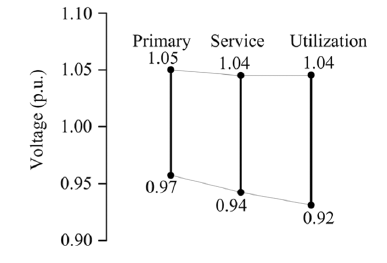
\includegraphics[width=0.5\linewidth]{imagenes/cap_1/rangos_tensiones}
%\end{figure}

El objetivo del sistema de potencia con relación al control de tensión es mantener mantenerla en un margenes en los diferentes nodos \cite{Liu2012}. 


\chapter{CONTROL DE TENSIÓN BASADO EN CAMBIADORES DE TOMAS}
\label{cap_oltc} 

\section{CARGADOR DE TOMAS BAJO CARGA}

El cambiador de taps bajo carga  ( \textit{On load Tap Changer } OLTC) es un tipo de auto transformador el cual esta localizado al interior del transformador de distribución y  se emplea para compensar las caídas de voltaje  a través del DS \cite{Castro2016}. En la figura \ref{fig:esquema_OLTC} se muestra el esquema general del OLTC en el cual $V_{1}$ es la tensión de entrada  y $V_{2}$ la de salida. El bloque  de control se encarga de conmutar los interruptores $sw_{1}$ a $sw_{n}$ de acuerdo a un algoritmo propio establecido por el \textit{operador de red} OR.\\\\
\begin{figure}[h]
    \centering
    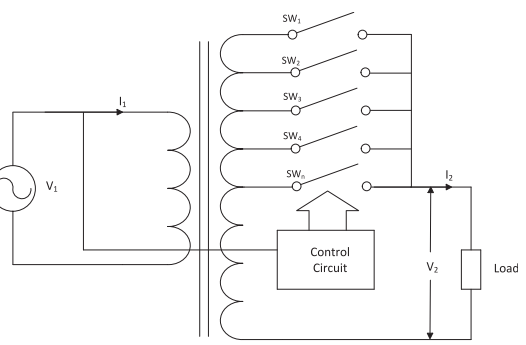
\includegraphics[width=0.6\linewidth]{imagenes/cap_1/Selection_275}
    \caption{Esquema general del cambiador de tap bajo carga \cite{Castro2016}}
    \label{fig:esquema_OLTC}
\end{figure}
\subsection{Esquemas de Control para OLTC}
El equipo encargado de del operar el OLTC es conocido como AVG (\textit{Automatic Voltage Control}), el cual conmuta las sus derivaciones del transformador de acuerdo a la desviación que se presente con respecto al la tensión de referencia o tensión objetivo, esto se puede ilustrar en la figura \ref{fig:esqusema_LDC} \cite{Sarimuthu2016}. Este control debe asegurarse que el voltaje se encentre siempre por encima del nivel mínimo de tensión el cual decrece a lo largo del circuito \cite{Sarimuthu2016} para el caso de un circuito radial sin DG. Las  mediciones realizadas en la figura \ref{fig:esqusema_LDC} son usadas para calcular la caída de tensión en el nodo remoto, esta técnica es conocida como LDC (\textit{Load Drop Control}).\\\\

\begin{figure}[h]
\centering
\caption{Esquema de controlador para OLTC con LDC \cite{Sarimuthu2016}}
\label{fig:esqusema_LDC}
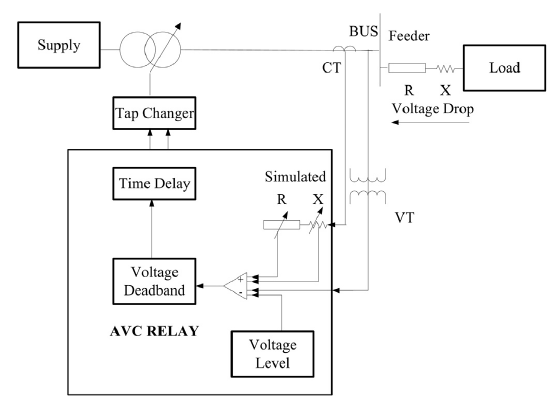
\includegraphics[width=0.7\linewidth]{imagenes/cap_2/LDC}
\end{figure}
El LDC emplea la para su operación una señal de voltaje  y otra de corriente con la cual  simula la caída de tensión (\textit{voltage drop})  en los parámetros internos R  y X \cite{Sarimuthu2016}. Una vez obtenido este valor  se compara con el ajuste deseado y de acuerdo al esquema de operación se aumenta disminuye o mantiene igual el tap del  transformador, tras esperar un tiempo de retardo ( \textit{time delay} ). El tiempo de retardo ( \textit{time delay} ) inicial esta alrededor de 10  a 120 s y el requerido entre cada paso  es de 5 a 60s  \cite{Sarimuthu2016}.\\\\

\paragraph{Coordinación en Tiempo}
En un sistema de potencia típico existen diversos AVG operando  en diversos niveles de tensión, lo cual hace que si operan de manera simultanea el sistema se comporte de manera inestable \cite{Sarimuthu2016}, por tanto  se hace necesario  establecer un esquema de coordinación entre los AVG. Esta coordinación debe realizarse de modo tal que el AVG aguas arriba tenga la prioridad  frente al que opera aguas abajo (en un menor nivel de tensión).
Este esquema puede implementarse por dos vías, una es ajustando  un retardo en el tiempo ( \textit{time delay})de conmutación del AVG o implementando una red de comunicación entre los dispositivos operados aguas arriba y aguas abajo, sin embargo esta ultima solución resulta costosa y presenta fallos tras presentarse anomalías en la comunicación \cite{Sarimuthu2016}. Por ello se emplean preferiblemente esquemas temporizados que incluyan las excepciones  de prioridad como las zonas de banda muerta en la operación del AVG \cite{Sarimuthu2016}.\\\\
\paragraph{Coordinación Maestro-Esclavo}
Este esquema opera con transformadores conectados en paralelo,  entonces el transformador maestro ajusta el tap en la posición deseada  y el transformador o transformadores esclavos se ajustan a la misma posición \cite{Fila2007}\cite{Sarimuthu2016}. 
\paragraph{Coordinación por método de circulación de corriente} 
Cuando dos transformadores son conectados en paralelo como se muestra en la figura \ref{fig:paralelo}, aparece una  corriente $I_{c}$ dado que la impedancia equivalente de cada transformador no es exactamente la misma \cite{Fila2007}.\\\\
\begin{figure}[h]
\centering
\caption{Control de tensión de transformadores en paralelo con OLTC}
\label{fig:paralelo}
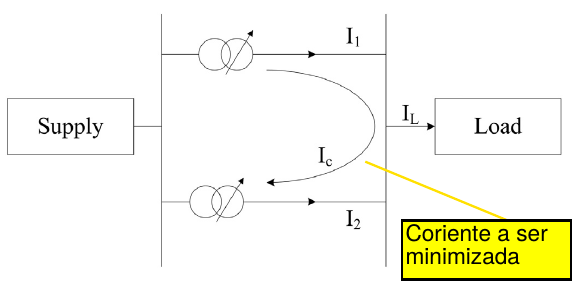
\includegraphics[width=0.7\linewidth]{imagenes/cap_2/paralelo}
\end{figure}
Esta corriente  de circulación esta dada por:\\\\
\begin{equation}
  \label{eq:icir}
I_{cir} = \dfrac{I_{T1} - I_{T2}}{2} 
\end{equation}
Para el transformador con el tap más alto $I_{c}$ es positiva, mientras que para el  otro es negativa. Cada uno AVC asociado a un transformador emplea un sistema de comunicación para conocer el valor de la corriente del otro. Esta corriente $I_{c}$ es convertida en cada uno de los AVC en una tensión de ajuste.
\paragraph{Coordinación por medio de la reactancia negativa}
En este esquema los transformadores en paralelo parten del mismo tap, cambiando solamente el signo del parámetro reactancia dentro del AVC.La principal ventaja de este método es que no requiere de comunicación en entre los AVC.
\begin{figure}[h]
\centering
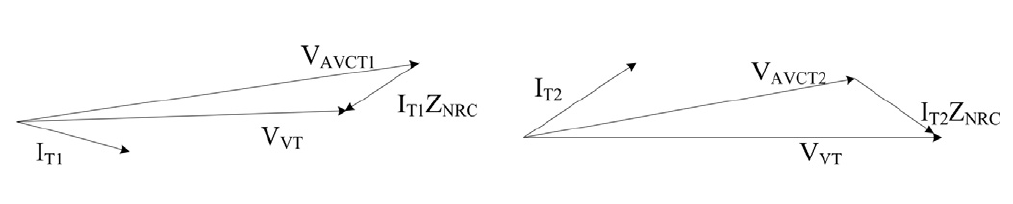
\includegraphics[width=0.7\linewidth]{imagenes/cap_2/diagrama_fasorial_nrc}
\caption{Diagrama fasorial NRC}
\label{fig:diagrama_fasorial_nrc}
\end{figure}
Para explicar el funcionamiento del NRC, se muestra el diagrama fasorial de la figura \ref{fig:diagrama_fasorial_nrc}, en esta el transformador T1 tiene una posición más alta en el tap por lo que la corriente fluye desde el T1 al T2\cite{Sarimuthu2016}. Debido a la corriente de circulación ($I_{cir}$) las corrientes $I_{T1}$ e $I_{T2}$  están desfasadas. En cada AVC es computado el valor $I_{T} \bullet Z_{NRC}$ como una caída de tensión la cual se suma con el ajuste de tensión objetivo $V_{T}$ para obtener la tensión para cada AVC $V_{AVCT}$. Si esta tensión es superior a la tensión de referencia $V_{T}$, entonces es decrementada  la posición del tap \cite{Sarimuthu2016}.

\section{REGULADOR DE TENSIÓN}
Otro dispositivo similar al este es el SRV (\textit{Step Regulator Voltage})

\section{CONTROL AUTOMÁTICO DE TENSIÓN}


\chapter{CONTROL DE TENSIÓN BASADO EN LA REGULACIÓN DE POTENCIA ACTIVA Y REACTIVA}
\label{cap_reactiva}

\cite{Oshiro2011}
\chapter{CONTROL DE TENSIÓN BASADO EN EL ALMACENAMIENTO DE ENERGÍA}
\label{cap_almacenamiento}
\chapter{CONTROL DE TENSIÓN BASADO EN EL CONTROL DEL INVERSOR }
\label{cap_inversor}
\chapter{CONTROL DE TENSIÓN CENTRALIZADO}
\label{cap_central}
\chapter{COORDINACIÓN Y PLANEACIÓN  DEL SISTEMA DE DISTRIBUCIÓN PARA LA LOCALIZACION OPTIMA DE LA GENERACIÓN DISTRIBUIDA }


\label{cap_planeacion}
\cite{Idlbi2013}

% Bibliografía
\bibliographystyle{ieeetr}
\bibliography{library,bibliografia_anteproyecto}
%\bibliographystyle{ieeetr}

\end{document}
